\resizebox{\textwidth}{!}{
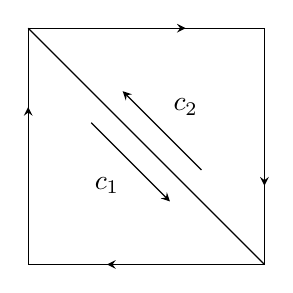
\begin{tikzpicture}
\draw (0,0) -- (0,3) -- (3,3) -- (3,0) -- cycle;

\draw[-stealth] (0,1) -- (0,2);
\draw[-stealth] (1,3) -- (2,3);
\draw[-stealth] (3,2) -- (3,1);
\draw[-stealth] (2,0) -- (1,0);

\draw (1,1) node {$c_1$};
\draw (2,2) node {$c_2$};

\draw (3,0) -- (0,3);
\draw[-stealth] (1-1/5,2-1/5) -- (2-1/5,1-1/5);
\draw[stealth-] (1+1/5,2+1/5) -- (2+1/5,1+1/5);
\end{tikzpicture}
}